\chapter{Metodología, herramientas y arquitectura general}
\label{cap:metodologia}

El Capítulo~\ref{cap:ecosistema_cvn} analizó el contenido real del paquete
oficial CVN, identificó sus limitaciones técnicas y presentó, a un nivel
todavía conceptual, la arquitectura por capas que Open CVN propone frente a
esas limitaciones. El presente capítulo desciende un nivel de concreción:
describe el proceso de trabajo seguido durante el desarrollo, justifica la
selección de herramientas empleadas y detalla la arquitectura general del
sistema, incluida la organización del repositorio que la materializa. Los
detalles de implementación de cada capa se reservan para el
Capítulo~\ref{cap:pipeline}.

\section{Metodología de trabajo}
\label{sec:metodologia_proceso}

El desarrollo de este Trabajo Fin de Grado no siguió un proceso de ingeniería
del software orientado a requisitos de usuario o iteraciones de producto, sino
un proceso adaptado a un trabajo de Computación centrado en el análisis de
formatos, la generación reproducible de artefactos y la verificación técnica de
un sistema. Este proceso puede describirse en cinco fases sucesivas.

La primera fase consistió en un análisis inicial del dominio curricular y de
los formatos de representación disponibles, cuyo resultado se recoge en el
Capítulo~\ref{cap:estado_arte}. La segunda fase exploró en detalle los
artefactos oficiales del paquete CVN, identificando su estructura y sus
limitaciones técnicas, tal y como se presentó en el
Capítulo~\ref{cap:ecosistema_cvn}. La tercera fase, desarrollada en el presente
capítulo, diseñó de forma incremental una arquitectura por capas capaz de
absorber esas limitaciones sin perder trazabilidad hacia las fuentes
oficiales. La cuarta fase implementó dicha arquitectura de forma reproducible,
generando de manera automática los artefactos estructurales, los metadatos
normalizados, los modelos de dominio y el formato Open CVN JSON, como se
describe en el Capítulo~\ref{cap:pipeline}. La quinta fase verificó el
sistema mediante pruebas automatizadas y flujos completos de extremo a
extremo, cuyos resultados se discuten en el Capítulo~\ref{cap:evaluacion}.

Estas cinco fases no se ejecutaron de forma estrictamente secuencial. Cada
limitación detectada durante la exploración del paquete oficial obligó, en la
práctica, a revisar decisiones de diseño ya tomadas en fases anteriores, y cada
nueva capa incorporada exigió documentar explícitamente las decisiones y las
limitaciones que introducía. Esta documentación continua de decisiones y
limitaciones técnicas, más que una fase aislada, constituye un criterio
transversal de todo el proceso: ninguna limitación detectada se resolvió
ocultándola, sino registrándola y decidiendo de forma explícita cómo debía
tratarse en la capa correspondiente.

\section{Herramientas empleadas}
\label{sec:metodologia_herramientas}

La selección de herramientas responde a un criterio común: cada herramienta
debía permitir generar o validar artefactos de forma reproducible a partir de
fuentes formales, sin introducir dependencias que condicionaran en exceso la
portabilidad del sistema.

El proyecto se implementa en Python, cuya combinación de tipado gradual y
ecosistema maduro de procesamiento de XML y JSON resulta adecuada para
implementar las sucesivas capas de generación y transformación descritas en
este documento. La gestión del entorno y de las dependencias se realiza con
\textit{uv}, un gestor de paquetes y proyectos Python que permite fijar de
forma determinista tanto la versión del intérprete como las dependencias
empleadas~\cite{uv_docs}, un requisito necesario para que la generación de
artefactos sea reproducible entre distintos entornos de ejecución.

La generación de la capa estructural a partir de los esquemas XSD oficiales se
realiza con \textit{xsdata}, una biblioteca de generación de enlaces de datos
que permite obtener clases Python tipadas directamente desde esquemas XML sin
necesidad de traducirlos manualmente~\cite{xsdata_docs}. Esta herramienta se
complementa con su extensión para Pydantic, que emite las clases generadas ya
como modelos Pydantic en lugar de estructuras de datos genéricas.

Pydantic actúa como base de los modelos de dominio, del formato Open CVN JSON y
de buena parte de la validación en tiempo de ejecución del sistema. Como ya se
introdujo en el Capítulo~\ref{cap:estado_arte}, Pydantic combina anotaciones de
tipo, validación de datos y generación de JSON Schema en un mismo
mecanismo~\cite{pydantic_docs}, lo que permite mantener alineados el código
Python, el contrato de validación y la documentación estructural del formato.
Ese contrato de validación se expresa como JSON Schema, cuya versión Draft
2020-12 es la empleada para validar de forma declarativa el formato Open CVN
JSON antes de aplicar las comprobaciones adicionales en tiempo de
ejecución~\cite{json_schema_overview}.

El almacenamiento local de currículos, versiones y diagnósticos se apoya en
SQLite, un motor de bases de datos embebido que no requiere un servidor
independiente~\cite{sqlite_docs}. Esta elección evita introducir una
dependencia de infraestructura externa y mantiene la herramienta local
autocontenida. La exportación a documentos LaTeX se implementa con Jinja, un
motor de plantillas que separa la lógica de presentación de los datos ya
validados~\cite{jinja_docs}, de modo que la generación de un documento LaTeX no
exige mezclar código Python con marcado de presentación.

La verificación automatizada del sistema se realiza con \textit{pytest} como
marco de pruebas, junto con su extensión \textit{pytest-xdist} para la
ejecución en paralelo de la batería de pruebas~\cite{pytest_docs}, lo que
permite mantener tiempos de ejecución razonables a pesar del volumen de
comprobaciones necesarias para cubrir las distintas capas del sistema. El
control de versiones se realiza con Git, y cada contribución se verifica de
forma automática mediante GitHub Actions, un servicio de integración continua
que ejecuta la batería de pruebas ante cualquier cambio propuesto sobre el
repositorio~\cite{github_actions_docs}.

La Tabla~\ref{tab:metodologia_herramientas} resume estas herramientas junto con
su papel principal y la justificación de su uso dentro del proyecto.

\begin{table}[htbp]
  \centering
  \footnotesize
  \renewcommand{\arraystretch}{1.55}
  \caption{Herramientas empleadas en el proyecto y justificación de su uso.}
  \label{tab:metodologia_herramientas}
  \begin{tabular}{p{0.22\textwidth} p{0.34\textwidth} p{0.32\textwidth}}
    \hline
    \textbf{Herramienta} & \textbf{Papel en el proyecto} & \textbf{Justificación} \\
    \hline
    Python + \textit{uv} & Lenguaje de implementación y gestión reproducible del entorno y las dependencias & Tipado gradual, ecosistema maduro para XML/JSON y fijación determinista del entorno de ejecución \\
    \textit{xsdata} + extensión Pydantic & Generación de bindings estructurales desde los esquemas XSD oficiales & Evita traducir manualmente esquemas complejos y mantiene los bindings alineados con la fuente oficial \\
    Pydantic & Modelos de dominio, formato Open CVN JSON y validación en tiempo de ejecución & Combina tipado, validación y generación de JSON Schema en un mismo mecanismo \\
    JSON Schema (Draft 2020-12) & Validación estructural declarativa del formato Open CVN JSON & Contrato de validación independiente del lenguaje de implementación \\
    SQLite & Almacenamiento local de currículos, versiones y diagnósticos & Motor embebido que evita una dependencia de infraestructura externa \\
    Jinja + motor LaTeX & Exportación de currículos almacenados a documentos LaTeX y PDF & Separa la plantilla de presentación de los datos ya validados \\
    \textit{pytest} + \textit{pytest-xdist} & Verificación automatizada y ejecución paralela de la batería de pruebas & Mantiene tiempos de ejecución razonables sobre una batería de pruebas extensa \\
    Git + GitHub Actions & Control de versiones e integración continua & Verifica automáticamente cada contribución antes de integrarse \\
    \hline
  \end{tabular}
\end{table}

\section{Arquitectura general por capas}
\label{sec:metodologia_arquitectura}

La arquitectura general del sistema traduce en artefactos concretos la
separación conceptual presentada en el Capítulo~\ref{cap:ecosistema_cvn} entre
el paquete oficial CVN y el modelo Open CVN derivado de él. La
Figura~\ref{fig:metodologia_arquitectura} representa esta arquitectura
agrupada en cuatro grandes bloques, cada uno de los cuales corresponde a una
parte concreta del repositorio del proyecto.

\begin{figure}[htbp]
  \centering
  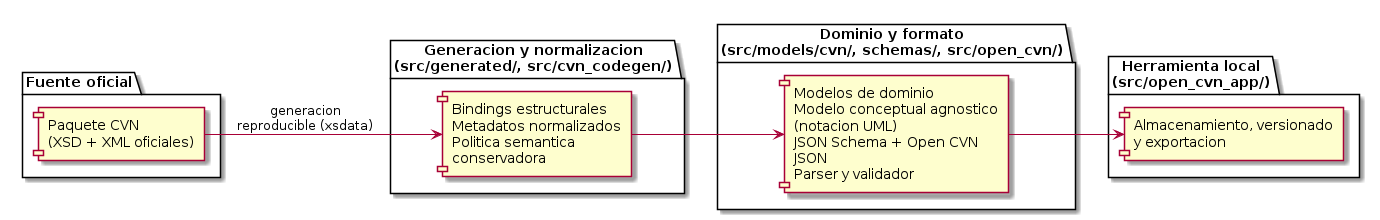
\includegraphics[width=0.95\textwidth]{figs/open_cvn_layered_architecture.png}
  \caption{Arquitectura general de Open CVN organizada por capas, con el módulo del repositorio responsable de cada bloque.}
  \label{fig:metodologia_arquitectura}
\end{figure}

Cada uno de estos cuatro bloques agrupa, a su vez, una secuencia de etapas más
concretas. Los apartados siguientes describen esa secuencia bloque a bloque,
indicando para cada etapa qué recibe, qué produce y qué módulo del repositorio
la implementa. El detalle interno de cómo se implementa cada etapa, incluidos
los algoritmos y los resultados numéricos de su ejecución, se reserva para el
Capítulo~\ref{cap:pipeline}; este apartado se limita a establecer el mapa
general de responsabilidades entre etapas.

\subsection{Fuente oficial CVN}
\label{sec:metodologia_arquitectura_fuente}

El primer bloque no realiza ningún procesamiento propio: corresponde al
paquete oficial CVN ya descrito en el Capítulo~\ref{cap:ecosistema_cvn}, y
actúa como frontera externa y única fuente formal de la que parte el resto de
la arquitectura. Ninguna etapa posterior incorpora información curricular que
no proceda, directa o indirectamente, de este bloque.

\subsection{Generación estructural y normalización}
\label{sec:metodologia_arquitectura_generacion}

El segundo bloque transforma el paquete oficial en metadatos internos
normalizados y semánticamente interpretados, en cuatro etapas sucesivas:

\begin{itemize}
  \item \textbf{Generación estructural.} A partir de los esquemas XSD
  oficiales se generan de forma reproducible bindings Pydantic que reflejan
  fielmente la estructura del XML de CVN. Esta etapa produce los bindings
  estructurales almacenados en \texttt{src/generated/} y no incorpora todavía
  ninguna interpretación semántica de los campos.

  \item \textbf{Normalización.} A partir del manual funcional en XML y del
  modelo en árbol, esta etapa unifica en una única estructura, indexada por
  código CVN, la información hasta entonces dispersa entre ambas fuentes.
  Recibe el paquete oficial y produce metadatos normalizados por código.

  \item \textbf{Resolución de referencias auxiliares.} Sobre los metadatos
  normalizados, esta etapa resuelve las referencias del manual hacia las
  familias auxiliares del paquete descritas en el
  Capítulo~\ref{cap:ecosistema_cvn}, añadiendo a cada metadato la evidencia de
  resolución disponible.

  \item \textbf{Política semántica.} A partir de los metadatos ya resueltos,
  esta etapa decide de forma explícita y trazable la forma semántica de cada
  campo (texto, fecha, número, enumeración cerrada, catálogo abierto,
  referencia a entidad, término de tesauro o referencia no resuelta, entre
  otras), produciendo una política semántica completa del dominio.
\end{itemize}

Las cuatro etapas de este bloque se implementan como lógica mantenida a mano
en \texttt{src/cvn\_codegen/}, con la única excepción de los bindings
generados por la primera etapa, que se almacenan de forma separada en
\texttt{src/generated/}.

\subsection{Dominio, modelo conceptual y formato}
\label{sec:metodologia_arquitectura_dominio}

El tercer bloque construye, a partir de la política semántica, las
representaciones que ya no dependen de la estructura concreta del XML de CVN:

\begin{itemize}
  \item \textbf{Modelos de dominio.} A partir de la política semántica se
  generan modelos de dominio Pydantic, almacenados en \texttt{src/models/cvn/}
  junto con un conjunto reducido de componentes de dominio compartidos
  mantenidos a mano.

  \item \textbf{Modelo conceptual agnóstico.} A partir de los modelos de
  dominio y de las decisiones de normalización y política semántica que los
  originaron, esta etapa construye el inventario conceptual detallado en el
  Capítulo~\ref{cap:pipeline}, ya independiente de la serialización XML. Es
  precisamente este modelo conceptual, y no los modelos de dominio en
  Python ni el formato Open CVN JSON, el que se representa mediante
  diagramas de clases UML, tal y como se justificó en el
  Capítulo~\ref{cap:estado_arte} y se ilustró de forma compacta en la
  Figura~\ref{fig:ecosistema_uml_overview} del
  Capítulo~\ref{cap:ecosistema_cvn}: UML actúa como notación intermedia de
  este bloque, entre la política semántica que lo alimenta y los artefactos
  técnicos (JSON Schema, formato Open CVN JSON) que se derivan de él.

  \item \textbf{JSON Schema y formato Open CVN JSON.} A partir del modelo
  conceptual se genera el artefacto JSON Schema, almacenado en
  \texttt{schemas/}, que define de forma declarativa la estructura válida del
  formato Open CVN JSON.

  \item \textbf{Parser y validador.} Sobre el JSON Schema y los modelos de
  dominio se apoya el contrato público de análisis y validación, almacenado en
  \texttt{src/open\_cvn/}, que expone la importación de Open CVN JSON, CVN XML
  y CVN PDF junto con la validación en tiempo de ejecución.
\end{itemize}

Las tres primeras etapas de este bloque se mantienen en
\texttt{src/cvn\_codegen/} y \texttt{src/models/cvn/}; la última corresponde ya
al módulo \texttt{src/open\_cvn/}, que constituye el límite público del
sistema hacia cualquier código externo que necesite leer o validar currículos.

\subsection{Herramienta local}
\label{sec:metodologia_arquitectura_herramienta}

El cuarto bloque no añade una etapa de transformación de datos, sino que
consume el contrato público de análisis y validación para ofrecer un uso
operativo completo: inicialización de almacenamiento, importación y
exportación, gestión de un currículo maestro y de versiones derivadas,
selección de secciones y entradas, y exportación a LaTeX y PDF. Todo este
bloque se implementa en \texttt{src/open\_cvn\_app/}.

La Tabla~\ref{tab:metodologia_modulos} consolida, para cada módulo del
repositorio mencionado en los apartados anteriores, la responsabilidad que le
corresponde dentro de la arquitectura Open CVN.

\begin{table}[htbp]
  \centering
  \footnotesize
  \renewcommand{\arraystretch}{1.55}
  \caption{Módulos del repositorio y responsabilidades dentro de la arquitectura Open CVN.}
  \label{tab:metodologia_modulos}
  \begin{tabular}{p{0.24\textwidth} p{0.64\textwidth}}
    \hline
    \textbf{Módulo} & \textbf{Responsabilidad} \\
    \hline
    \texttt{src/generated/} & Bindings estructurales Pydantic generados automáticamente desde los esquemas XSD oficiales; no se edita manualmente \\
    \texttt{src/cvn\_codegen/} & Lógica mantenida a mano: normalización, resolución de referencias auxiliares, política semántica, generación de modelos de dominio, extracción del modelo conceptual y generación de diagramas y JSON Schema \\
    \texttt{src/models/cvn/} & Componentes de dominio compartidos mantenidos a mano y modelos de dominio generados automáticamente a partir de la política semántica \\
    \texttt{schemas/} & Artefacto JSON Schema generado del formato Open CVN \\
    \texttt{src/open\_cvn/} & Contrato público de análisis y validación: importación de Open CVN JSON, CVN XML y CVN PDF, y validación en tiempo de ejecución \\
    \texttt{src/open\_cvn\_app/} & Herramienta local: interfaz de línea de órdenes, almacenamiento SQLite, versionado, edición de selección y exportación a LaTeX y PDF \\
    \hline
  \end{tabular}
\end{table}

\section{Contratos entre capas y razonamiento arquitectónico}
\label{sec:metodologia_contratos}

La separación entre módulos descrita en el apartado anterior no es únicamente
organizativa: cada frontera entre módulos corresponde a un contrato explícito
que determina qué información puede cruzar de una capa a otra. Generar un
modelo de dominio final directamente desde los esquemas XSD oficiales, sin
capas intermedias, mezclaría dos preocupaciones de naturaleza distinta: la
interoperabilidad estructural con el XML de CVN y el modelado semántico del
dominio curricular. Por ello, los bindings estructurales generados
automáticamente se tratan como una capa de fidelidad hacia el XML oficial, y
cualquier limpieza semántica o ergonómica se realiza en capas posteriores, en
lugar de modificarse a mano sobre el código generado.

Esta decisión tiene una consecuencia práctica directa sobre la
reproducibilidad del sistema: dado que la capa estructural puede regenerarse en
cualquier momento a partir de los esquemas oficiales sin perder trabajo manual,
las limitaciones que dicha capa presenta, ya descritas en el
Capítulo~\ref{cap:ecosistema_cvn}, quedan documentadas en lugar de
enmascararse mediante ediciones manuales frágiles. De forma análoga, los
modelos de dominio y el modelo conceptual no vuelven a inspeccionar el XML o
los esquemas XSD originales, sino que consumen exclusivamente las decisiones ya
tomadas por la normalización y por la política semántica, evitando así que la
semántica del dominio se derive de forma inconsistente en distintos puntos del
sistema. El contrato público de análisis y validación, a su vez, expone
únicamente el formato Open CVN JSON y sus resultados de validación, sin
obligar a quien lo utiliza a conocer los detalles internos de generación de las
capas anteriores.

En conjunto, esta arquitectura por capas materializa de forma concreta la
propuesta presentada en el Capítulo~\ref{cap:ecosistema_cvn}: conserva
trazabilidad hacia el paquete oficial CVN en cada etapa, mantiene separadas la
interoperabilidad estructural y la semántica de dominio, y permite verificar de
forma independiente cada capa mediante pruebas automatizadas. El
Capítulo~\ref{cap:pipeline} describe en detalle cómo se implementa cada una
de estas capas, desde la
generación estructural hasta la extracción del modelo conceptual y la
generación de diagramas y JSON Schema.
